\documentclass[a4paper]{article}
\usepackage[a4paper, margin=1in]{geometry}
% Some basic packages
\usepackage[utf8]{inputenc}
\usepackage[T1]{fontenc}
\usepackage{textcomp}
\usepackage[dutch]{babel}
\usepackage{url}
\usepackage{graphicx}
\usepackage{float}
\usepackage{booktabs}
\usepackage{enumitem}

\pdfminorversion=7

% Don't indent paragraphs, leave some space between them
\usepackage{parskip}

% Hide page number when page is empty
\usepackage{emptypage}
\usepackage{subcaption}
\usepackage{multicol}
\usepackage{xcolor}

% Other font I sometimes use.
% \usepackage{cmbright}

% Math stuff
\usepackage{amsmath, amsfonts, mathtools, amsthm, amssymb}
% Fancy script capitals
\usepackage{mathrsfs}
\usepackage{cancel}
% Bold math
\usepackage{bm}
% Some shortcuts
\newcommand\N{\ensuremath{\mathbb{N}}}
\newcommand\R{\ensuremath{\mathbb{R}}}
\newcommand\Z{\ensuremath{\mathbb{Z}}}
\renewcommand\O{\ensuremath{\emptyset}}
\newcommand\Q{\ensuremath{\mathbb{Q}}}
\newcommand\C{\ensuremath{\mathbb{C}}}

% Easily typeset systems of equations (French package)
\usepackage{systeme}

% Put x \to \infty below \lim
\let\svlim\lim\def\lim{\svlim\limits}

%Make implies and impliedby shorter
\let\implies\Rightarrow
\let\impliedby\Leftarrow
\let\iff\Leftrightarrow
\let\epsilon\varepsilon

% Add \contra symbol to denote contradiction
\usepackage{stmaryrd} % for \lightning
\newcommand\contra{\scalebox{1.5}{$\lightning$}}

% \let\phi\varphi

% Command for short corrections
% Usage: 1+1=\correct{3}{2}

\definecolor{correct}{HTML}{009900}
\newcommand\correct[2]{\ensuremath{\:}{\color{red}{#1}}\ensuremath{\to }{\color{correct}{#2}}\ensuremath{\:}}
\newcommand\green[1]{{\color{correct}{#1}}}

% horizontal rule
\newcommand\hr{
    \noindent\rule[0.5ex]{\linewidth}{0.5pt}
}

% hide parts
\newcommand\hide[1]{}

% si unitx
\usepackage{siunitx}
\sisetup{locale = FR}

% Environments
\makeatother
% For box around Definition, Theorem, \ldots
\usepackage{mdframed}
\mdfsetup{skipabove=1em,skipbelow=0em}
\theoremstyle{definition}
\newmdtheoremenv[nobreak=true]{definitie}{Definitie}
\newmdtheoremenv[nobreak=true]{eigenschap}{Eigenschap}
\newmdtheoremenv[nobreak=true]{gevolg}{Gevolg}
\newmdtheoremenv[nobreak=true]{lemma}{Lemma}
\newmdtheoremenv[nobreak=true]{propositie}{Propositie}
\newmdtheoremenv[nobreak=true]{stelling}{Stelling}
\newmdtheoremenv[nobreak=true]{wet}{Wet}
\newmdtheoremenv[nobreak=true]{postulaat}{Postulaat}
\newmdtheoremenv{conclusie}{Conclusie}
\newmdtheoremenv{toemaatje}{Toemaatje}
\newmdtheoremenv{vermoeden}{Vermoeden}
\newtheorem*{herhaling}{Herhaling}
\newtheorem*{intermezzo}{Intermezzo}
\newtheorem*{notatie}{Notatie}
\newtheorem*{observatie}{Observatie}
\newtheorem*{oef}{Oefening}
\newtheorem*{opmerking}{Opmerking}
\newtheorem*{praktisch}{Praktisch}
\newtheorem*{probleem}{Probleem}
\newtheorem*{terminologie}{Terminologie}
\newtheorem*{toepassing}{Toepassing}
\newtheorem*{uovt}{UOVT}
\newtheorem*{vb}{Voorbeeld}
\newtheorem*{vraag}{Vraag}

\newmdtheoremenv[nobreak=true]{definition}{Definition}
\newtheorem*{eg}{Example}
\newtheorem*{notation}{Notation}
\newtheorem*{previouslyseen}{As previously seen}
\newtheorem*{remark}{Remark}
\newtheorem*{note}{Note}
\newtheorem*{problem}{Problem}
\newtheorem*{observe}{Observe}
\newtheorem*{property}{Property}
\newtheorem*{intuition}{Intuition}
\newmdtheoremenv[nobreak=true]{prop}{Proposition}
\newmdtheoremenv[nobreak=true]{theorem}{Theorem}
\newmdtheoremenv[nobreak=true]{corollary}{Corollary}

% End example and intermezzo environments with a small diamond (just like proof
% environments end with a small square)
\usepackage{etoolbox}
\AtEndEnvironment{vb}{\null\hfill$\diamond$}%
\AtEndEnvironment{intermezzo}{\null\hfill$\diamond$}%
% \AtEndEnvironment{opmerking}{\null\hfill$\diamond$}%

% Fix some spacing
% http://tex.stackexchange.com/questions/22119/how-can-i-change-the-spacing-before-theorems-with-amsthm
\makeatletter
\def\thm@space@setup{%
  \thm@preskip=\parskip \thm@postskip=0pt
}


% Exercise 
% Usage:
% \oefening{5}
% \suboefening{1}
% \suboefening{2}
% \suboefening{3}
% gives
% Oefening 5
%   Oefening 5.1
%   Oefening 5.2
%   Oefening 5.3
\newcommand{\oefening}[1]{%
    \def\@oefening{#1}%
    \subsection*{Oefening #1}
}

\newcommand{\suboefening}[1]{%
    \subsubsection*{Oefening \@oefening.#1}
}


% \lecture starts a new lecture (les in dutch)
%
% Usage:
% \lecture{1}{di 12 feb 2019 16:00}{Inleiding}
%
% This adds a section heading with the number / title of the lecture and a
% margin paragraph with the date.

% I use \dateparts here to hide the year (2019). This way, I can easily parse
% the date of each lecture unambiguously while still having a human-friendly
% short format printed to the pdf.

\usepackage{xifthen}
\def\testdateparts#1{\dateparts#1\relax}
\def\dateparts#1 #2 #3 #4 #5\relax{
    \marginpar{\small\textsf{\mbox{#1 #2 #3 #5}}}
}

\def\@lecture{}%
\newcommand{\lecture}[3]{
    \ifthenelse{\isempty{#3}}{%
        \def\@lecture{Lecture #1}%
    }{%
        \def\@lecture{Lecture #1: #3}%
    }%
    \subsection*{\@lecture}
    \marginpar{\small\textsf{\mbox{#2}}}
}



% These are the fancy headers
\usepackage{fancyhdr}
\pagestyle{fancy}

% LE: left even
% RO: right odd
% CE, CO: center even, center odd
% My name for when I print my lecture notes to use for an open book exam.
% \fancyhead[LE,RO]{Gilles Castel}

\fancyhead[RO,LE]{\@lecture} % Right odd,  Left even
\fancyhead[RE,LO]{}          % Right even, Left odd

\fancyfoot[RO,LE]{\thepage}  % Right odd,  Left even
\fancyfoot[RE,LO]{}          % Right even, Left odd
\fancyfoot[C]{\leftmark}     % Center

\makeatother




% Todonotes and inline notes in fancy boxes
\usepackage{todonotes}
\usepackage{tcolorbox}

% Make boxes breakable
\tcbuselibrary{breakable}

% Verbetering is correction in Dutch
% Usage: 
% \begin{verbetering}
%     Lorem ipsum dolor sit amet, consetetur sadipscing elitr, sed diam nonumy eirmod
%     tempor invidunt ut labore et dolore magna aliquyam erat, sed diam voluptua. At
%     vero eos et accusam et justo duo dolores et ea rebum. Stet clita kasd gubergren,
%     no sea takimata sanctus est Lorem ipsum dolor sit amet.
% \end{verbetering}
\newenvironment{verbetering}{\begin{tcolorbox}[
    arc=0mm,
    colback=white,
    colframe=green!60!black,
    title=Opmerking,
    fonttitle=\sffamily,
    breakable
]}{\end{tcolorbox}}

% Noot is note in Dutch. Same as 'verbetering' but color of box is different
\newenvironment{noot}[1]{\begin{tcolorbox}[
    arc=0mm,
    colback=white,
    colframe=white!60!black,
    title=#1,
    fonttitle=\sffamily,
    breakable
]}{\end{tcolorbox}}




% Figure support as explained in my blog post.
\usepackage{import}
\usepackage{xifthen}
\usepackage{pdfpages}
\usepackage{transparent}
\newcommand{\incfig}[1]{%
    \def\svgwidth{\columnwidth}
    \import{./figures/}{#1.pdf_tex}
}

% Fix some stuff
% %http://tex.stackexchange.com/questions/76273/multiple-pdfs-with-page-group-included-in-a-single-page-warning
\pdfsuppresswarningpagegroup=1

\title{\Huge{Probability 1 - Hw 1}}
\author{\huge{Daniel Yu}}
\date{September 13,2024}

\pdfsuppresswarningpagegroup=1

\begin{document}
\maketitle
\newpage% or \cleardoublepage
% \pdfbookmark[<level>]{<title>}{<dest>}
\pagebreak

\begin{enumerate}
  \item Prove $P(\cup_{i=1}^n A_i) \leq \sum_{i=1}^n P(A_i)$.
      \begin{proof}
        Let each event $A_i \subseteq \Omega$ and the set $\{A_i\}_{i \in 1,\ldots,n}$ be a finite collection of subsets of 
        $\Omega$. If each $A_i$ is disjoint, then we are done from the definition of a probability measure property 3. If
        $A_i$ is not disjoint, then there exists $x \in A_i \cap A_j$ for two distinct subsets $A_i,A_j$. Let the set
        $X = A_i \cap A_j$. Start with the base case where $n=2$ and there are two events $A_1, A_2$. Then, 
        $P(A_1 \cup A_2) = P(A_1 \setminus X \cup A_2 \setminus X \cup X) = P\left(A_1 \setminus X \cup A_2 \right) = P(A_1 \setminus X) 
        + P(A_2) \leq P(A_1) + P(A_2)$ since each of $A_1 \setminus X, A_2 \setminus X, X$ are disjoint sets by construction. Assume
        that the hypothesis holds for some $k$, $P(\cup_{i=1}^k A_i) \leq \sum_{i=1}^{k} P(A_i)$. Then for $k+1$, 
        $P(\cup_{i=1}^{k+1} A_i)= P(\cup_{i=1}^k A_i \cup A_{k+1})$. If $A_{k+1}$ is disjoint from  $\cup_{i=1}^k A_i$
        then  $P(\cup_{i=1}^k A_i \cup A_{k+1}) = P(\cup_{i=1}^k A_i) + P(A_{k+1}) \leq  \sum_{i=1}^{k} P(A_i) + P(A_{k+1})
        = \sum_{i=1}^{k+1} P(A_i)$ and we are done. If $A_{k+1}$ is not disjoint, then a similar argument as from the base case
        holds. Take $X = A_{k+1} \cap \cup_{i=1}^k A_i$. Then,
        $P(\cup_{i=1}^{k} A_i \cup A_{k+1}) = P(\cup_{i=1}^{k} A_i \setminus X \cup A_{k+1} \setminus X \cup X) = 
        P(\cup_{i=1}^{k} A_i \cup A_{k+1} \setminus X) = P(\cup_{i=1}^k A_i) + P(A_{k+1} \setminus X) \leq \sum_{i=1}^k P(A_i) + P(A_{k+1} \setminus X) 
        \leq  \sum_{i=1}^k P(A_i) + P(A_{k+1}) = \sum_{i=1}^{k+1} P(A_i)$. QED
      \end{proof}
    \item What is the value of $c_1,c_2$?
      \begin{note}
      
        \begin{align*}
          \int_{-\infty}^{\infty}  f_X(s) ds &= \int_{0}^{4} \frac{c_1}{\sqrt{s}} + c_{2}s ds\\
                                             &= [2 c_1 s^{\frac{1}{2}} + \frac{1}{2}c_2 s^2]_0^4 \\
                                             &= 2 \cdot 2 \cdot c_1 + 8 \cdot c_2 \\
                                             &= 1
        .\end{align*}
        We are also given:
        \[
          P[X \leq 1] = \frac{1}{3} 
        .\] 
        So,
        \begin{align*}
          P[X \leq 1] = \int_{0}^1 f_X(s) ds &= [2 c_1 s^{\frac{1}{2}} + \frac{1}{2}c_2 s^2]_0^1 \\
                                             &= 2 \cdot c_1 + \frac{1}{2} \cdot c_2 \\
                                             &= \frac{1}{3}
        .\end{align*}
        Solving the system and substituting $c_2 = \frac{2}{3} - 4 c_1$:
        \begin{align*}
          4 \cdot c_1 + 8 \cdot c_2 &= 4 \cdot c_1 + 8 \cdot (\frac{2}{3} - 4c_1) \\
                                    &= 4c_1 + \frac{16}{3} - 32c_1 \\
                                    &= -28c_1 + \frac{16}{3} \\
                                    &= 1
        .\end{align*}
        \[
        c_1 = \frac{13}{84}
        .\] 
        and,
        \[
        c_2 =\frac{1}{21}
        .\]      

      \end{note}
    \item Let $N$ be a random variable that takes non-negative integer values. Show 
      \[
        E[N] = \sum_{n=1}^\infty P[N \geq n]
      .\] 
      \begin{proof}
        \begin{align*}
          \sum_{n=1}^\infty P[N \geq n] &= P[N \geq 1] + P[N \geq 2] + P[N \geq 3] + \ldots \\
                                        &= (P[N=1] + P[N=2] + P[N=3] + \ldots) + (P[N = 2] + P[N=3] + \ldots) + (P[N = 3] + \ldots) + \ldots + 0 \\
                                        &= P[N=1] + 2P[N=2] + 3P[N=3] + \ldots + \sum_{n=1}^k P[n=k] + \ldots \\
                                        &= \sum_{k=1}^\infty \sum_{n=1}^k P[N=k] \\
                                        &= \sum_{k \in range(N)} k P[n=k] \\
                                        &= E[N]
        .\end{align*}
      \end{proof}
    \item Consider two random variables $X,Y$:
      \begin{enumerate}
        \item What is the probability that $X=Y$?
          \begin{note}
            We know that $P[X=2, Y=3] + P[X=2, Y=1] + P[X=2, Y=2] = P[X=2] = \frac{1}{3}$ 
            and $P[X=2, Y=2] + P[X=1, Y=2] + P[X=3, Y=2] = P[Y=2] = \frac{1}{3}$. Substituting in the give values:
            \[
              \frac{1}{12} + P[X=2, Y=1] + P[X=2, Y=2] = \frac{1}{3}
            .\] 
            \[
              P[X=2, Y=2] + P[X=1,Y=2] + \frac{1}{4} = \frac{1}{3}
            .\]
            We also know $P[X=1, Y=1] + P[X=2, Y=1] + P[X=3, Y=1] = P[Y=1] = \frac{1}{3}$ and 
            $P[X=1, Y=1] + P[X=1, Y=2] + P[X=1, Y=3] = P[X=1] = \frac{1}{3}$.
            \[
              \frac{1}{12} + P[X=2, Y=1] + P[X=3,Y=1] = \frac{1}{3}
            .\] 
            \[
              \frac{1}{12} + P[X=1,Y=2] + P[X=1, Y=3] = \frac{1}{3}
            .\]. Finally, we know:
            \[
              P[X=3, Y=1] + \frac{1}{4} + P[X=3, Y=3] = \frac{1}{3}
            .\] 
            \[
              P[X=1, Y=3] + \frac{1}{12} + P[X=3, Y=3] = \frac{1}{3}
            .\]
            There are 6 equations and 6 unknowns, so we can solve this 
            linear system.

\begin{figure}[H]
  \centering
  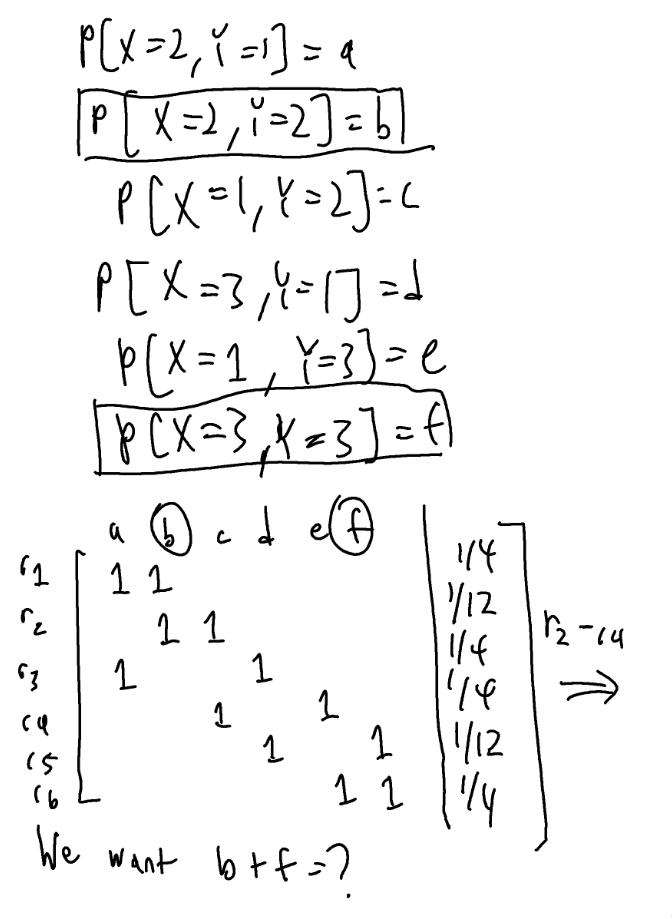
\includegraphics[width=0.8\textwidth]{assets/2024-09-13-16-16-34.png}
  \caption{}
  \label{fig:2024-09-13-16-16-34}
\end{figure}

\begin{figure}[H]
  \centering
  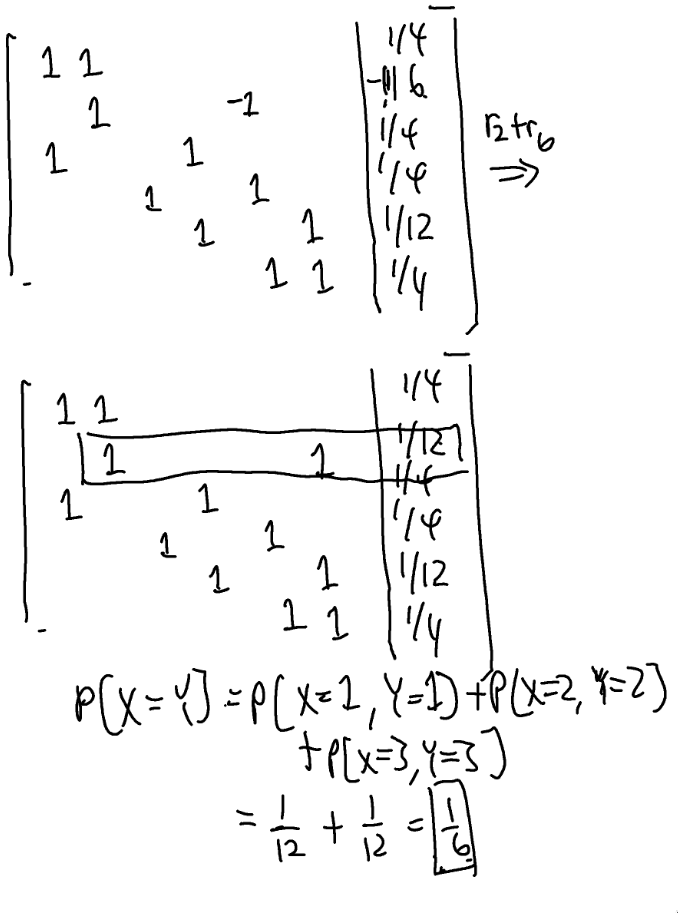
\includegraphics[width=0.8\textwidth]{assets/2024-09-13-16-16-51.png}
  \caption{}
  \label{fig:2024-09-13-16-16-51}
\end{figure}
          Note that the matrix is not full rank and the rows and columns of the 
          matrix are not linearly independent!
          \end{note}
        \item What is the smallest possible value of $P[X=2, Y=1]$.
        \begin{note}
          From the matrix we can extract the following equations where $P[x=2,Y=1] = a$
           \[
          a + b = \frac{1}{4}
          .\] 
          \[
          b + f = \frac{1}{12}
          .\] 
          We know that probabilities have to be non-negative so $a,b,c,d,e,f \geq 0$. Given this
          constraint, let  $f = 0$, then maximum possible value for b is:
           \[
          b + 0 = \frac{1}{12} \to b= \frac{1}{12}
          .\] 
          and 
          \[
          a + \frac{1}{12} = \frac{1}{4} \to a=\frac{1}{6}
          .\] 
          Thus, the smallest possible value of $a = \frac{1}{6}$.
        \end{note}
        
      \end{enumerate}
   \item Consider stick of length $1$. We break along a uniformly chosen point on the stick. Let $L$ be the longer 
          piece's length:
          \begin{enumerate}
            \item What is the PDF $f_L(s)$?
              \begin{note}
                Start by considering the CDF: $F_L(s) = P[L \leq s]$ where $s$ could be any value for the
                length of the longer piece. First, notice that since it is the length of the longer piece,
                $L \geq .5$ and $s \geq .5$. So,
                \[
                F_L(s) = \begin{cases}
                  P[L \leq s], 1 \geq s \geq .5 \\
                  0, \text{otherwise}
                \end{cases}
                .\] 
                Imagine the stick as the interval $[0,1]$. If we choose the point at the distance $.1$ as the cut or 
                the point at the distance $.9$ as the cut, the length of the longer piece would still be $.9$. In 
                fact over the entire interval $[.1,.9]$, the length of the longer piece $L \leq .9$. Since we
                know that the stick is distributed uniformly along the interval $[0,1]$,
                \[
                F_L(s) = \begin{cases}
                  \frac{s - (1-s)}{1} = 2s - 1, 1 \geq s \geq .5 \\
                  0, \text{ otherwise}
                \end{cases} 
                .\]
                Then to take the pdf, we would simply take the first derivative:
                \[
                \frac{d}{ds} F_L(s) = \frac{d}{ds}( 2s - 1) = 2
                .\]. 
                Thus, the pdf would simply be 
                \[
                f_L(s) = \begin{cases}
                  2, 1 \geq s \geq .5 \\
                  0, \text{otherwise}
                \end{cases}
                .\] 
              \end{note}
             \item What is the expected value of $L$?
                \[
                  E[L] = \int_{-\infty}^{\infty} s \cdot f_L(s) ds =  \int_{.5}^{1} s \cdot 2 ds = [s^2]_{.5}^1  
                .\] 
                \[
                = .75
                .\] 
              \item What is the variance of $L$?
                \begin{align*}
                  var(L) &= E[L^2] - (E[L])^2  \\
                         &= \int_{-\infty}^{\infty} s^2 \cdot f_L(s) ds - (.75)^2 \\
                         &= \int_{.5}^1 s^2 \cdot 2 - .5625 \\
                         &= [\frac{2}{3}s^3]_{.5}^1 - .5625 \\
                         &= [\frac{2}{3} - \frac{1}{12}] - .5625 \\
                         &= \frac{1}{48}
                .\end{align*}
            \end{enumerate}
\end{enumerate}
\end{document}
